\documentclass{beamer}
\usepackage{tfrupee} 
\usepackage[utf8]{inputenc}
\usepackage{lmodern} 
\usepackage{listings}
\usepackage{xcolor} 
\usepackage{graphicx}
\usepackage{amsmath,amssymb,amsfonts}

\definecolor{myblue}{RGB}{48, 63, 159}
\setbeamercolor{palette primary}{bg=myblue, fg=white}
\setbeamercolor{structure}{fg=myblue}
\setbeamercolor{frametitle}{bg=myblue, fg=white}
\setbeamercolor{title}{bg=myblue, fg=white}
\setbeamercolor{footlinecolor}{bg=myblue, fg=white}

\defbeamertemplate*{title page}{mytemplate}{
	\vfill
	\begin{center}
		\begin{beamercolorbox}[wd=0.8\paperwidth, center, rounded=true, shadow=true]{title}
			\usebeamerfont{title}\inserttitle\par
		\end{beamercolorbox}
		\vspace{2cm} 
		\usebeamerfont{author}\insertauthor
		\vspace{1cm} 
		\usebeamerfont{date}\insertdate
	\end{center}
	\vfill
}

\defbeamertemplate*{frametitle}{mytemplate}{
	\begin{beamercolorbox}[wd=\paperwidth, ht=2.5ex, dp=1.5ex, left]{frametitle}
		\hspace{1em}\usebeamerfont{frametitle}\insertframetitle
	\end{beamercolorbox}
}

\setbeamertemplate{footline}{
	\begin{beamercolorbox}[wd=\paperwidth, ht=2.25ex, dp=1ex]{footlinecolor}
		\hspace{1em}\usebeamerfont{author in footline}\insertshortauthor
		\hfill
		\usebeamerfont{title in footline}\insertshorttitle
		\hfill
		\usebeamerfont{date in footline}\insertdate \hspace{1em} \insertframenumber/\inserttotalframenumber \hspace{0.5em}
	\end{beamercolorbox}
}

\setbeamerfont{author in footline}{size=\tiny}
\setbeamerfont{title in footline}{size=\tiny}
\setbeamerfont{date in footline}{size=\tiny}

\newcommand{\myvec}[1]{\ensuremath{\begin{pmatrix}#1\end{pmatrix}}}
\providecommand{\brak}[1]{\ensuremath{\left(#1\right)}}

\title{10.6.8 - Eigenvector Method}
\author{Shriyansh Chawda-EE25BTECH11052}

\begin{document}
	
	\setbeamertemplate{footline}{} 
	\frame{\titlepage}
	
	\begin{frame}{Question} 
		Construct a pair of tangents to a circle of radius 4cm from a point P lying outside the circle at 
		a distance of 6cm from the centre.
		\hfill{(10, 2023)}\\
	\end{frame}
	
	\begin{frame}{Problem Setup}
		Let the center of the circle be at origin and point P be at distance 6 from center along x-axis.
		\begin{align}
			O &= \myvec{0\\0}\\
			P &= \myvec{6\\0}
		\end{align}
		
		The equation of the circle $x^2 + y^2 = 16$ can be written as:
		\begin{equation}
			\vec{x}^\top \vec{V} \vec{x} + 2\vec{u}^\top \vec{x} + f = 0
		\end{equation}
		where
		\begin{equation}
			\vec{V} = \myvec{1 & 0\\0 & 1}, \quad \vec{u} = \myvec{0\\0}, \quad f = -16
		\end{equation}
	\end{frame}
	
	\begin{frame}{Step 1: Eigenvalue Decomposition}
		The eigenvalues of $\vec{V}$ satisfy:
		\begin{align}
			\det(\vec{V} - \lambda\vec{I}) &= 0\\
			(1-\lambda)^2 &= 0
		\end{align}
		
		\textbf{Eigenvalues:} $\lambda_1 = \lambda_2 = 1$
		
		\vspace{1em}
		The corresponding orthonormal eigenvectors are:
		\begin{equation}
			\vec{p}_1 = \myvec{1\\0}, \quad \vec{p}_2 = \myvec{0\\1}
		\end{equation}
		
		These form the eigenvector matrix:
		\begin{equation}
			\vec{P} = \myvec{\vec{p}_1 & \vec{p}_2} = \myvec{1 & 0\\0 & 1}
		\end{equation}
	\end{frame}
	
	\begin{frame}{Step 2: Semi-axes from Eigenvalues}
		The semi-axes of the circle along eigenvector directions:
		\begin{equation}
			a = b = \sqrt{\frac{-f}{\lambda_1}} = \sqrt{\frac{16}{1}} = 4
		\end{equation}
		
		\vspace{1em}
	\end{frame}
	
	\begin{frame}{Step 3: Tangency Conditions}
		For tangents from external point $P$ to the circle, the contact point $\vec{q}$ must satisfy:
		\begin{enumerate}
			\item[(a)] $\vec{q}$ lies on circle: $\vec{q}^\top\vec{V}\vec{q} + f = 0$
			\item[(b)] Tangent passes through $P$: $(\vec{V}\vec{q})^\top P + f = 0$
		\end{enumerate}
		
		\vspace{1em}
		From condition (b) with $\vec{V} = \vec{I}$:
		\begin{align}
			\vec{q}^\top P + f &= 0\\
			\myvec{q_1 & q_2}\myvec{6\\0} &= 16\\
			q_1 &= \frac{8}{3}
		\end{align}
	\end{frame}
	
	\begin{frame}{Step 4: Finding Contact Points}
		From condition (a):
		\begin{align}
			q_1^2 + q_2^2 &= 16\\
			\brak{\frac{8}{3}}^2 + q_2^2 &= 16\\
			q_2 &= \pm\frac{4\sqrt{5}}{3}
		\end{align}
		
		Therefore, the two contact points are:
		\begin{equation}
			\vec{q}_1 = \myvec{\frac{8}{3}\\\frac{4\sqrt{5}}{3}}, \quad \vec{q}_2 = \myvec{\frac{8}{3}\\-\frac{4\sqrt{5}}{3}}
		\end{equation}
	\end{frame}
	
	\begin{frame}{Step 5: Eigenvector Representation}
	Express contact points as linear combinations of eigenvectors:
		\begin{align}
			\vec{q}_1 &= \frac{8}{3}\vec{p}_1 + \frac{4\sqrt{5}}{3}\vec{p}_2\\
			&= \frac{8}{3}\myvec{1\\0} + \frac{4\sqrt{5}}{3}\myvec{0\\1}\\
			&= \myvec{\frac{8}{3}\\\frac{4\sqrt{5}}{3}}
		\end{align}
		
		\begin{align}
			\vec{q}_2 &= \frac{8}{3}\vec{p}_1 - \frac{4\sqrt{5}}{3}\vec{p}_2\\
			&= \myvec{\frac{8}{3}\\-\frac{4\sqrt{5}}{3}}
		\end{align}
	
	\end{frame}
	
	\begin{frame}{Step 6: Tangent Equations}
		The tangent at $\vec{q}$ is given by: $(\vec{V}\vec{q})^\top \vec{x} + f = 0$
		
		\vspace{1em}
		\textbf{Tangent 1} at $\vec{q}_1$:
		\begin{align}
			\myvec{\frac{8}{3} & \frac{4\sqrt{5}}{3}}\myvec{x\\y} - 16 &= 0\\
			\frac{8}{3}x + \frac{4\sqrt{5}}{3}y &= 16\\
			2x + \sqrt{5}y &= 12
		\end{align}
		
		\textbf{Tangent 2} at $\vec{q}_2$:
		\begin{align}
			\myvec{\frac{8}{3} & -\frac{4\sqrt{5}}{3}}\myvec{x\\y} - 16 &= 0\\
			2x - \sqrt{5}y &= 12
		\end{align}
	\end{frame}
	
	\begin{frame}{Final Answer}
		The equations of the pair of tangents are:
		\begin{equation}
			\boxed{2x + \sqrt{5}y = 12 \quad \text{and} \quad 2x - \sqrt{5}y = 12}
		\end{equation}
	\end{frame}
	
	
	
	\begin{frame}{Plot}
		\begin{figure}[H]
			\centering
			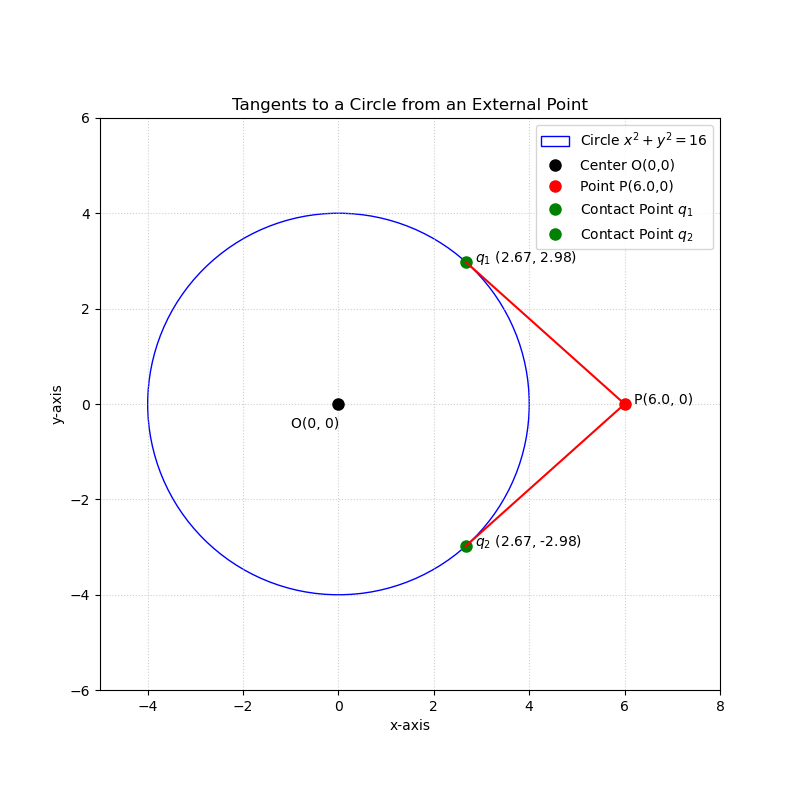
\includegraphics[width=0.85\linewidth]{figs/tangents_plot}
			\caption{Circle with tangents from external point P}
			\label{fig:tangentsplot}
		\end{figure}
	\end{frame}
	
\end{document}